\begin{figure*}
  \centering
  \begin{subfigure}[b]{0.42\textwidth}
    \centering
    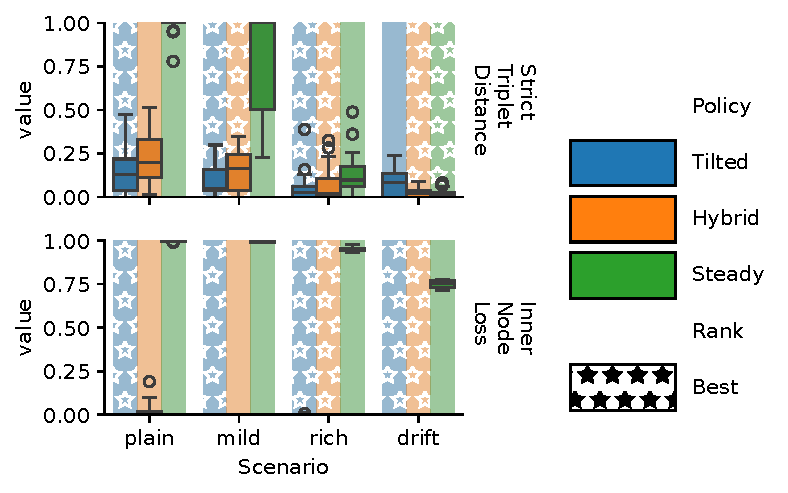
\includegraphics[width=\textwidth]{binder/binder/steady-vs-tilted/teeplots/annotation-size-bits=64+differentia-width-bits=1+downsample=500+hue=policy+num-generations=100000+population-size=65536+row=variable+score=value+viz=peckplot+x=scenario+x-group=outer+y=value+ext=}
    \caption{Example reconstruction quality distributions. Lower is better.}
    \label{fig:steady-vs-tilted-summary-example}
  \end{subfigure}%
  \begin{subfigure}[b]{0.58\textwidth}
    \centering
    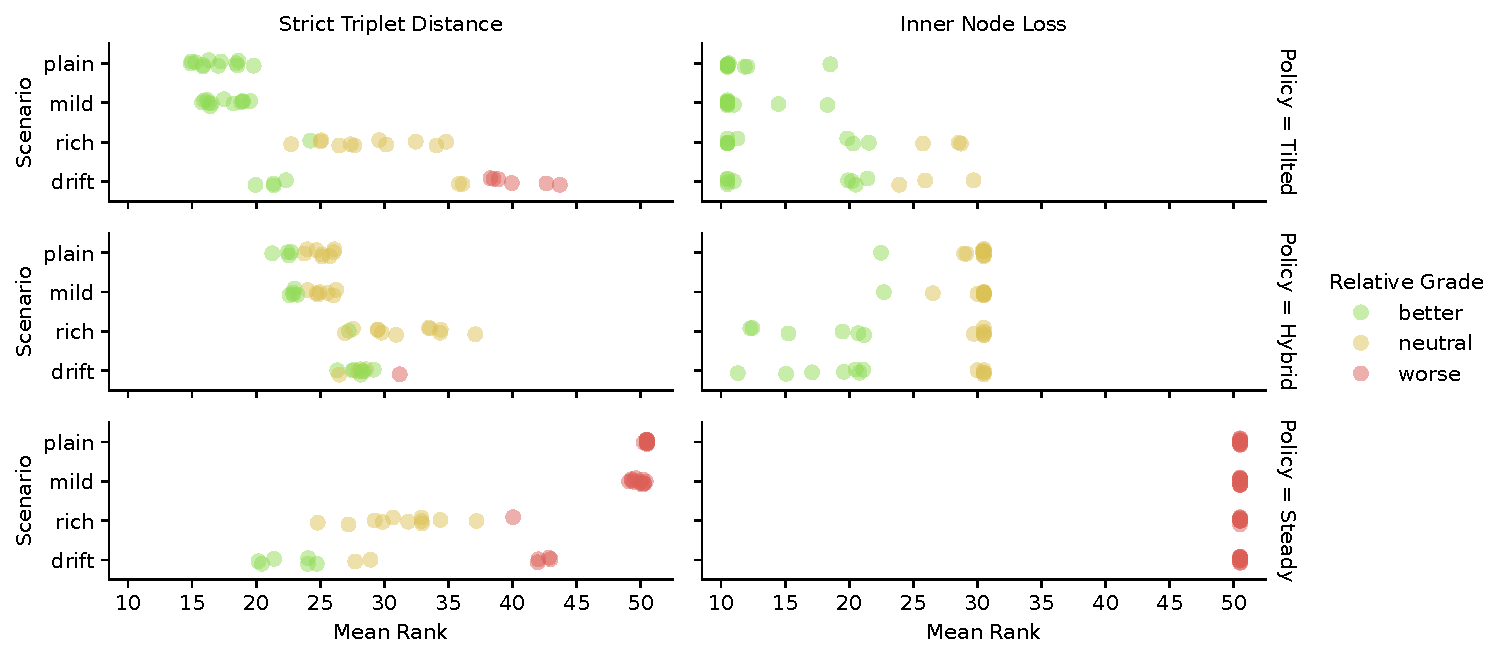
\includegraphics[width=\textwidth]{binder/binder/steady-vs-tilted/teeplots/col=metric+hue=relative-grade+kind=strip+row=policy+viz=catplot+x=mean-rank+y=scenario+ext=}
    \caption{Reconstruction quality comparison outcomes. Lower is better.}
    \label{fig:steady-vs-tilted-summary-overview}
  \end{subfigure}
  \caption{%
    \textbf{How does retention policy affect reconstruction quality?}
    \footnotesize
    Subpanel \ref{fig:steady-vs-tilted-summary-overview} shows mean rank among reconstruction error measures from tilted, hybrid, and steady retention policies across sensitivity analysis conditions.
    Each point represents an independent 20-replicate trial under different evolutionary conditions, instrumentation configuration (e.g., annotation size), and phylogenetic scale (e.g., reconstruction tip count).
    Color coding indicates significant outcome (Kruskal-Wallis H then Mann-Whitney U test).
    Lower is better.
    Tilted policy (top row) performs best in most evolutionary scenarios, except triplet distance under the highly phylogenetically-rich drift regime.
    Steady policy (bottom row) performs worst in most scenarios, except triplet distance under the drift regime.
    Hybrid policy performance has somewhat higher triplet distance reconstruction distance error in the plain and mild scenarios than tilted policy, but is robust to the drift regime.
    Subpanel \ref{fig:steady-vs-tilted-summary-example} shows reconstruction quality effects for 64-bit size, bit-differentia annotations with population size 65,536, downsample size 500, and 100k generations.
    Background hagching indicates significant outcome.
    See Supplementary Figure \ref{fig:steady-vs-tilted} for listing of reconstruction quality outcomes by sensitivity analysis condition.
  }
  \label{fig:steady-vs-tilted-summary}
\end{figure*}
